%% For double-blind review submission
\documentclass[acmlarge,review,anonymous]{acmart}\settopmatter{printfolios=true}
%% For single-blind review submission
%\documentclass[acmlarge,review]{acmart}\settopmatter{printfolios=true}
%% For final camera-ready submission
%\documentclass[acmlarge]{acmart}\settopmatter{}

%% Note: Authors migrating a paper from PACMPL format to traditional
%% SIGPLAN proceedings format should change 'acmlarge' to
%% 'sigplan,10pt'.


%% Some recommended packages.
\usepackage{booktabs}   %% For formal tables:
                        %% http://ctan.org/pkg/booktabs
\usepackage{subcaption} %% For complex figures with subfigures/subcaptions
                        %% http://ctan.org/pkg/subcaption


% AMS packages
\usepackage{amsmath}
\usepackage{amssymb}
\usepackage{amsthm}
\usepackage{mathtools}
\usepackage{mdwlist}

% Hyper links
\usepackage{url}
\usepackage{hyperref}
\hypersetup{
   colorlinks,
   citecolor=black,
   filecolor=black,
   linkcolor=black,
   urlcolor=black
}

% Miscellaneous
\usepackage{paralist}
\usepackage{graphicx}
\usepackage{float}

% Code highlighting
\usepackage{listings}

% Revision tools
\usepackage{xspace}
\usepackage{xcolor}
\usepackage{comment}
\newcommand{\hltext}[2][gray!40]{\colorbox{#1}{#2}}
\newcommand{\hl}[2][gray!40]{%
  \colorbox{#1}{$\displaystyle#2$}}
\newcommand{\mynotes}[3]{{\color{#2} {\sc #1}: #3}}
\newcommand\bruno[1]{\mynotes{bruno}{red}{#1}}
\newcommand\jeremy[1]{\mynotes{jeremy}{blue}{#1}}

\makeatletter\if@ACM@journal\makeatother
%% Journal information (used by PACMPL format)
%% Supplied to authors by publisher for camera-ready submission
\acmJournal{PACMPL}
\acmVolume{1}
\acmNumber{1}
\acmArticle{1}
\acmYear{2017}
\acmMonth{1}
\acmDOI{10.1145/nnnnnnn.nnnnnnn}
\startPage{1}
\else\makeatother
%% Conference information (used by SIGPLAN proceedings format)
%% Supplied to authors by publisher for camera-ready submission
\acmConference[PL'17]{ACM SIGPLAN Conference on Programming Languages}{January 01--03, 2017}{New York, NY, USA}
\acmYear{2017}
\acmISBN{978-x-xxxx-xxxx-x/YY/MM}
\acmDOI{10.1145/nnnnnnn.nnnnnnn}
\startPage{1}
\fi


%% Copyright information
%% Supplied to authors (based on authors' rights management selection;
%% see authors.acm.org) by publisher for camera-ready submission
\setcopyright{none}             %% For review submission
%\setcopyright{acmcopyright}
%\setcopyright{acmlicensed}
%\setcopyright{rightsretained}
%\copyrightyear{2017}           %% If different from \acmYear


%% Bibliography style
\bibliographystyle{ACM-Reference-Format}
%% Citation style
%% Note: author/year citations are required for papers published as an
%% issue of PACMPL.
\citestyle{acmauthoryear}   %% For author/year citations



\begin{document}

%% Title information
\title[Short Title]{Full Title}         %% [Short Title] is optional;
                                        %% when present, will be used in
                                        %% header instead of Full Title.
\titlenote{with title note}             %% \titlenote is optional;
                                        %% can be repeated if necessary;
                                        %% contents suppressed with 'anonymous'
\subtitle{Subtitle}                     %% \subtitle is optional
\subtitlenote{with subtitle note}       %% \subtitlenote is optional;
                                        %% can be repeated if necessary;
                                        %% contents suppressed with 'anonymous'


%% Author information
%% Contents and number of authors suppressed with 'anonymous'.
%% Each author should be introduced by \author, followed by
%% \authornote (optional), \orcid (optional), \affiliation, and
%% \email.
%% An author may have multiple affiliations and/or emails; repeat the
%% appropriate command.
%% Many elements are not rendered, but should be provided for metadata
%% extraction tools.

%% Author with single affiliation.
\author{First1 Last1}
\authornote{with author1 note}          %% \authornote is optional;
                                        %% can be repeated if necessary
\orcid{nnnn-nnnn-nnnn-nnnn}             %% \orcid is optional
\affiliation{
  \position{Position1}
  \department{Department1}              %% \department is recommended
  \institution{Institution1}            %% \institution is required
  \streetaddress{Street1 Address1}
  \city{City1}
  \state{State1}
  \postcode{Post-Code1}
  \country{Country1}
}
\email{first1.last1@inst1.edu}          %% \email is recommended

%% Author with two affiliations and emails.
\author{First2 Last2}
\authornote{with author2 note}          %% \authornote is optional;
                                        %% can be repeated if necessary
\orcid{nnnn-nnnn-nnnn-nnnn}             %% \orcid is optional
\affiliation{
  \position{Position2a}
  \department{Department2a}             %% \department is recommended
  \institution{Institution2a}           %% \institution is required
  \streetaddress{Street2a Address2a}
  \city{City2a}
  \state{State2a}
  \postcode{Post-Code2a}
  \country{Country2a}
}
\email{first2.last2@inst2a.com}         %% \email is recommended
\affiliation{
  \position{Position2b}
  \department{Department2b}             %% \department is recommended
  \institution{Institution2b}           %% \institution is required
  \streetaddress{Street3b Address2b}
  \city{City2b}
  \state{State2b}
  \postcode{Post-Code2b}
  \country{Country2b}
}
\email{first2.last2@inst2b.org}         %% \email is recommended


%% Paper note
%% The \thanks command may be used to create a "paper note" ---
%% similar to a title note or an author note, but not explicitly
%% associated with a particular element.  It will appear immediately
%% above the permission/copyright statement.
\thanks{with paper note}                %% \thanks is optional
                                        %% can be repeated if necesary
                                        %% contents suppressed with 'anonymous'


%% Abstract
%% Note: \begin{abstract}...\end{abstract} environment must come
%% before \maketitle command
\begin{abstract}
Text of abstract \ldots.
\end{abstract}


%% 2012 ACM Computing Classification System (CSS) concepts
%% Generate at 'http://dl.acm.org/ccs/ccs.cfm'.
\begin{CCSXML}
<ccs2012>
<concept>
<concept_id>10011007.10011006.10011008</concept_id>
<concept_desc>Software and its engineering~General programming languages</concept_desc>
<concept_significance>500</concept_significance>
</concept>
<concept>
<concept_id>10003456.10003457.10003521.10003525</concept_id>
<concept_desc>Social and professional topics~History of programming languages</concept_desc>
<concept_significance>300</concept_significance>
</concept>
</ccs2012>
\end{CCSXML}

\ccsdesc[500]{Software and its engineering~General programming languages}
\ccsdesc[300]{Social and professional topics~History of programming languages}
%% End of generated code


%% Keywords
%% comma separated list
\keywords{keyword1, keyword2, keyword3}  %% \keywords is optional


%% \maketitle
%% Note: \maketitle command must come after title commands, author
%% commands, abstract environment, Computing Classification System
%% environment and commands, and keywords command.
\maketitle

%% -- Starting Point --


\section{Introduction}

Mainstream statically-typed Object-Oriented Programming (OOP) languages (such as Java,
C++ C\# or Scala) all use a similar programming model based on
classes. For the remainder of the paper this will be referred to as
the \emph{standard model}. The standard model has its roots on the
origins of OOP in the 1960's in the Simula~\cite{} language. 
The standard model essentially provides a \emph{covariant} view of
objects, where the following basic properties are expected:
\bruno{are the two below essentially the same?}

\begin{itemize}

\item {\bf Extensions produce subtypes:} In the standard model, when a 
subclass \emph{extends} a class it automatically becomes a 
\emph{subtype} of the super-class. 

\item{\bf Inheritance and subtyping go along together:}
Class extension does two things at once: it inherits code from the
superclass; and it creates a subtype. In other words inheritance and
subtyping always go along together. 

\end{itemize}

The standard model has been sucessefully being used for over 50 years,
so it clearly has demonstrated its value in practice. In our personal
opinion this success can be attributed to a few things. Firstly,
subtyping and inheritance enable forms of reusability and modularity 
that are not easily or naturally available in languages without such
mechanisms. Secondly, the model is relatively simple and intuitive 
to grasp for programmers. \bruno{more?}

Unfortunatelly the study of the theoretical foundations has
taught us that the story about OOP is not quite so simple. Since the
earliest works on the theory of OOP and subtyping, we have known that 
the covariant view of objects is somewhat simplified. 

Cardelli's work on calculi for OOP has shown, for example, that
functions are not strictly covariant.  A function of type $A \to B$ is
a subtype of another function $C \to D$ when $B$ is a subtype of $D$
and $A$ is a \emph{supertype} of $C$. This means, for example that a
function of type $Cat \to Int$ \emph{cannot not be subtype} of a
function with type $Animal \to Int$ (assumming that $Cat$ is a subtype
of $Animal$). In fact, only the opposite can
happen: $Animal \to Int$ can be a subtype of $Cat \to Int$.  This is
at odds with the covariant view. Mainstream OOP languages such as Java or C\# address this
disturbance of the covariant view by making methods \emph{invariant} on 
their argument types. In other words, if a class $A$ with method $m$
extends a class $B$ with method $m$, then $A.m$ can only override 
$B.m$ if the parameters types in both method signatures are \emph{exactly 
the same}. Thus mainstream OOP languages restrict the natural subtyping of
functions. Various other issues related to covariance are known. 
For example...

Cook et al.'s work on ``\emph{Inheritance is not Subtyping}''~\cite{}
is another example of how the theory of  OOP languages contradicts 
the simple covariant model. As Cook et al. argued inheritance and
subtyping are different relations: subtyping being a relation on types 
and inheritance being a relation on objects. In the standard model 
the subtype relation is based on the inheritance hierarchy. This 
would work very well if extensions would \emph{always} produce 
subtypes. However, as Cook et al.'s work famously demonstrated 
this is not always the case. Following their observations about 
inheritance and subtyping, Cook et al. suggest a programing model 
with the following properties:

\begin{itemize}

\item {\bf Inheritance and subtyping should be decoupled:} 
That is, there should be different mechanisms for class inheritance 
and class/interface subtyping. 

\item {\bf Extensions do not always produce subtypes:} 
There are cases where classes can inherit from other classes without 
producing subtypes. 

\end{itemize}

Therefore Cook et al's model does away with the simple-minded covariant 
view of objects, and proposes a more general model

Despite being proposed almost 30 years ago, and one of the most
famous papers in OOP, Cook et al.'s paper has not had much impact 
on the design of OOP languages. A possible explanation for this 


There are multiple flavours of inheritance. To avoid confusion, since 
the same terminology is often used in the literature to mean different 
things, we use the following 3 terms in this paper:

\begin{itemize}



\item{{\bf Static inheritance:}} Static inheritance refers to what the
  typical model of inheritance in class-based languages. The
  inheritance model is said to be static because when using class
  extension, the extended classes are statically known at compile-type.
Static inheritance is used in languages such as Java, Scala or C\# or
C++\footnote{Note that C++ templates allow the Mixin pattern, which
  enables ...}.

\item{{\bf Mutable Inheritance:}} Prototype-based languages such as 
Javascript or Self allow another model of inheritance, which we call
\emph{mutable inheritance}. In this inheritance model, self references 
can be changed at any point. 

\item{{\bf Dynamic Inheritance:}} Dynamic inheritance is a less well-known 
model which stands in between static and mutable inheritance.
Dynamic inheritance is a model used by some academic delegation 
OOP languages, such as ...  
Unlike the static inheritance model, with dynamic inheritance 
objects can inherits from other objects which are not statically
known. However, unlike mutable inheritance, the self-reference is not 
mutable and cannot be arbitrarely changed at run-time. 

\end{itemize}



\section{A Critique of Mainstream Class-Based OOP}

This section discusses several points about mainstream OOP languages
that work against modularity. 

\subsection{No Contravariant Subtyping on Arguments}

Simple example that illustrates this. Need an example with contravariant arguments

\subsection{No Separation Between Inheritance and Subtyping}

Example: visitors. 

\subsection{No Dynamic Inheritance}

Example: find good example? Design patterns?

\subsection{No Multiple Inheritance of Same Class}

Example: composing Object Algebras (can relate to visitors).

\section{Desugaring}
\label{sec:desugar}


The section provides the procedures of desugaring traits to \bname. The idea
behind trait translation is inspired by the functional mixin semantics using
open recursion, which is proposed by~\citet{cook1989denotational} in an untyped
setting. However, our translation is done in the context of a statically-typed
programming language, which is exactly why conflicts can be \textit{statically}
detected in traits.

\subsection{Trait Declarations}

Essentially traits are translated into term declarations, with methods becoming
record fields. The self-reference is adjusted to be the last parameter of the
declaration. For example,
\begin{lstlisting}
  trait point(x : Int, y: Int) { self : Point =>
    def x() = x
    def y() = self.x()
  }
\end{lstlisting}
becomes
\begin{lstlisting}
  def point (x : Int) (y : Int) (self : Point) =
  { x = \_ -> x
  , y = \_ -> self.x()
  }
\end{lstlisting}

Now it is clear that \lstinline{self} is not a special keyword: it can
have any name.

More formally, a trait of the form
\begin{lstlisting}[mathescape=true]
  trait m [$A_1$, ..., $A_n$] ($x_1 : A_1$, ..., $x_n : A_n$) inherits $a_1$ & ... & $a_n$ { s : $A_0$ =>
    def $m_1$(...) = $e_1$
    ...
    def $m_n$(...) = $e_n$
  }
\end{lstlisting}
is translated into a term declaration of the form
\begin{lstlisting}[mathescape=true]
  def m $A_1$ ... $A_n$ $(x_1 : A_1)$ ... $(x_n : A_n)$ $(s : A_0)$ = $a_1$(s) ,, ... ,, $a_n$(s) ,,
  {
    $m_1$ = \(...) -> $e_1$
  , ...
  , $m_n$ = \(...) -> $e_n$
  }
\end{lstlisting}


\subsection{Instantiations of Traits}

\name allows creating a single object from one or more traits. Specifically,
\lstinline{new} instantiates a trait by taking the fixpoint of its
corresponding open term. In fact, \lstinline{new} is translated as an inlined
fixpoint. For example,
\begin{lstlisting}
  new[Point] point(3,4)
\end{lstlisting}
becomes
\begin{lstlisting}
  let self : Point = point 3 4 self in self
\end{lstlisting}
Essentially the open term is closed using \textit{lazy fixpoints}. Lazy
fixpoints are a standard way to encode dynamic mixin inheritance and bind
self-reference in denotational semantics~\cite{cook1989denotational}.

Lazy fixpoints are implemented in \name using the built-in \lstinline{let}
construct (possibly recursive), which employs call-by-name semantics. It is
possible to choose call-by-value, then the type of the self-reference would
becomes a thunk, that is, \lstinline$T -> Point$.

The composition of traits in the \lstinline{new} expression is desugared using
the merge operator. Now it is clear that the reason traits have conflict
detection for free is that the merge operator is enforcing two terms being
merged are disjoint. For example,
\begin{lstlisting}
  new[Point & Norm] point(3,4) & euclideanNorm()
\end{lstlisting}
is turned into
\begin{lstlisting}
  let self : Point & Norm = (point 3 4 self) ,, (euclideanNorm () self) in self
\end{lstlisting}

Formally, a \lstinline{new} expression of the form
\begin{lstlisting}[mathescape=true]
  new[$A_1$ & ... & $A_n$] $a_1$ & ... & $a_n$
\end{lstlisting}
is translated into a let expression of the form
\begin{lstlisting}[mathescape=true]
  let self : $A_1$ & ... & $A_n$ = $a_1$(self) ,, ... ,, $a_n$(self) in self
\end{lstlisting}

\subsection{The Type for Traits}

\lstinline[mathescape=true]{Trait[$T_1, T_2$]} denotes the type of those traits
which provide an interface described by the type $T_2$ with dependency on $T_1$.
In fact, it is just like a type constructor except for the fact that it is
built-in in the language, and that the encoding is not exposed to the
programmers.

Formally, a trait type of the form \lstinline[mathescape=true]{Trait[$T_1, T_2$]} becomes \lstinline[mathescape=true]{$T_1$ -> $T_2$}.

\subsection{Record System}

Following~\citet{reynolds1997design} and~\citet{castagna1995calculus}, \name
leverages intersection types to type extensible records. The idea is that a
multi-field record can be encoded as merges of single-field records, and
multi-record types as intersections. Therefore in \name, there are only
single-field record constructs. As such, record operations in \name can occur on
\textit{any} type.

\subsubsection{Record Operations}

To illustrate the various operations on records, we consider a record with three
fields:
\begin{lstlisting}
  {open : Int, high : Int, low : Int}
\end{lstlisting}
Note that this type is just syntactic sugar for:
\begin{lstlisting}
  {open : Int} & {high : Int} & {low : Int}
\end{lstlisting}
That is, a multi-field record type is desugared as intersections of single-field
record types.

\name supports three primitive operations related to records:
\textit{construction} \textit{selection} and \textit{restriction}.
\textit{Extension}, described in many other record systems, is delegated to the
merge operator. Working with records is type-safe: the type system prevents
accessing a field that does not exist.

\paragraph{Record construction.} The usual notation for constructing records
\begin{lstlisting}
  {open = 192, high = 195, low = 189}
\end{lstlisting}
is a shorthand for merges of single-field records
\begin{lstlisting}
  {open = 192} ,, {high = 195} ,, {low = 189}
\end{lstlisting}

\paragraph{Record selection.} Fields are extracted using the dot notation. For
example,
\begin{lstlisting}
  {open = 192, high=195, low= 189}.open
\end{lstlisting}
selects the value of the field labelled \lstinline{open} from the record. Since
records are just merges of terms, we can even select a field that is buried deep
inside a merge, so long as it is present.
\begin{lstlisting}
  ({open = 192} ,, 3 ,, {low = 189}).open
\end{lstlisting}

\jeremy{say something about record restriction}

\paragraph{Record extension} Extension, just like construction, is implemented
with the merge operator. The following example adds a \lstinline{close} field to
the record:
\begin{lstlisting}
  {open = 192, high=195, low=189} ,, {close = 195}
\end{lstlisting}


\begin{comment}
\subsubsection{Restriction via Subtyping}

Unlike most record systems, restriction is not a primitive operation in \name.
Instead, \name uses subtyping for restriction. Combined with disjoint
quantification, we can encode a \lstinline{remove} function that removes a given
field from a record:
\lstinputlisting[linerange=5-5]{../examples/record.txt}% APPLY:linerange=RCD_DEF
\lstinline{remove} takes a value x which contains a record of type
\lstinline${low : Int}$ as well as some extra information of type \lstinline{B}.
The disjointness constraint ensures that the value of type \lstinline{B} does
not contain a record with type \lstinline${low : Int}$. The following examples
shows removing the \lstinline{low} field:
\lstinputlisting[linerange=10-11]{../examples/record.txt}% APPLY:linerange=RCD_EG
\end{comment}


\subsubsection{Disjointness of Records}

Most record calculi forbid duplicate labels in the declarations of record types.
Some allow labels coincide but the last field overrides the previous ones.
Records in \name allow duplicate labels. This is because we adopt a lenient
approach to record disjointness~\cite{alpuimdisjoint}. Of course records with
distinct fields are disjoint naturally. \name accepts duplicate labels as long
as the types of the overlapping fields are disjoint. For example,
\begin{lstlisting}
  {open = 192, high = 195, open = true}
\end{lstlisting}
is allowed in \name. An interesting question arises when we try to select a
duplicate label, say \lstinline{open}. What should be the result? Should it be
192 or \lstinline{true}? Neither choice is satisfying, as with the coherence
problem for merges. Instead \name rejects such expression, and asks for more
type information from the context. Thus the following is accepted because there
is only one \lstinline{open} associated with \lstinline{Int}.
\begin{lstlisting}
  {open = 192, high = 195, open = true}.open + 3
\end{lstlisting}

\section{Implementation}

The \name prototype implementation is structured around a typed core language
(\bname with some extensions). The main component of the implementation is an
elaborating type-checker, which takes a \bname expression, checks it, and
produces another expression in the target language. The final expression is then
directly executed by an interpreter. We chose call-by-name untyped lambda
calculus as the target language. Since we focus on the implementation, and types
are irrelevant after type checking, untyped lambda calculus is a suitable choice
with minimal syntax. With some simple optimization, the interpreter delivers
reasonably good execution efficiency.

The overall implementation is unremarkable, as it closely follows the semantics
that was presented by~\citet{alpuimdisjoint}. The whole pipeline is shown in
Figure~\ref{fig:pipeline}. The desugaring phase (cf. Section~\ref{sec:desugar})
takes a simple abstract data type (AST) generated by the parser, and returns a
\bname expression. Trait-related constructs disappear after this phase. The
type checking phase then takes a \bname expression from the previous phase, it
infers and checks its type, and in the meantime, produces an expression in the
target language. The type checker is the most involved component in the
pipeline. It contains a (coercive) subtyping procedure and a disjointness
checker, both of which are the most essential parts for \name to work as we
wanted it. The target expression (pure untyped lambda calculus) then enters the
final phase, and is executed by a simple interpreter.

The prototype implementation is written in just 1400 lines of Haskell code.

\begin{figure}
  \centering
  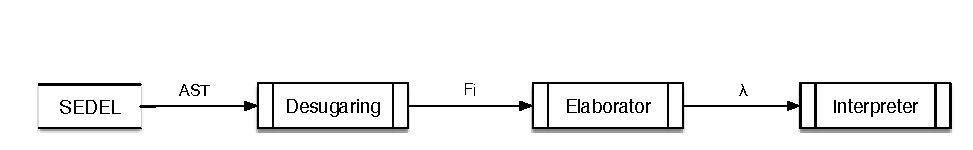
\includegraphics[scale=0.9]{pipeline.eps}
  \caption{The pipeline of \name}
  \label{fig:pipeline}
\end{figure}

\section{Related Work}

\begin{figure}[t]
  \centering
  \begin{tabular}{l|ccccc}
    \hline
     & \bf{Statically typed} & \bf{Polymorphism} & \bf{Covariant model} & \bf{Dynamic inheritance}  \\
    \hline
    \name & \cmark & \cmark & \xmark & \cmark \\
    \hline
    Scala & \cmark & \cmark & \cmark & \xmark \\
    \hline
    Java & \cmark & \cmark & \cmark & \xmark

  \end{tabular}
  \caption{Comparison between \name and various similar languages.}
  \label{fig:comparision}
\end{figure}


\subsection{(Disjoint) Intersection Types, Merge Operator}

There is a large body of work on studying intersection types. Dating back to
works as early as~\citet{coppo1981functional} and~\citet{pottinger1980type},
their motivation was to use intersection types to characterize exactly all
strongly normalizing lambda terms. Forsythe~\cite{reynolds1997design} is
probably the first practical programming language based on intersection types.
Since then various programming languages, including
CDuce~\cite{benzaken2003cduce}, Stardust~\cite{Dunfield07:Stardust}, Microsoft's
TypeScript, Redhat's Ceylon, Facebook's Flow, and Scala~\cite{scala-overview}
have incorporated some notion of intersection types.

The merge operator was first introduced in the Forsythe
language~\cite{reynolds1997design}. Recent work
by~\citet{dunfield2014elaborating} shows significant expressiveness of type
systems with intersection types and a merge operator. However their languages
all lack a important and desirable property of coherence. The limitation was
addressed by~\citet{oliveira2016disjoint}, where they introduce the notion of
disjointness to ensure coherence.

Previous work on incorporating polymorphism with intersection types includes
Pierce's $F_\wedge$~\cite{pierce1991programming2} and the recent work
by~\citet{Castagna:2014}. The former supports intersection types, polymorphism
and, as an extension, the merge operator. However $F_\wedge$ is incoherent due
to the use of such an extension. The latter is a coherent calculus with a
special merge operator that works on functions only. The \bname calculus,
proposed by~\citet{alpuimdisjoint} in their latest work, is the first coherent
calculus that includes parametric polymorphism, intersection types and a merge
operator. \bname serves the theoretical foundation of \name.


\subsection{Mainstream Languages with Delegation Mechanism}

\begin{itemize}
\item Clojure Protocols
  % http://www.ibm.com/developerworks/library/j-clojure-protocols/
\item Ruby mixin
\item JS mixin
\end{itemize}

They are all dynamically typed.

\subsection{Statically typed Delegation-based Languages}

\citet{cook1989inheritance} are the first to propose a typed model of
inheritance where subtyping and inheritance are two separate concepts. In
particular, they introduce the notion of \textit{type inheritance} and show that
inherited objects have inherited types, not subtypes. An interesting aspect of
their model is the \textbf{with} construct, used to join two records. This is
somewhat similar to our merge construct. However two major differences are worth
pointing out: 1) the \textbf{with} construct operates only on records, and 2) it
is a biased operation, meaning the conflict is resolved by favoring values from
its right argument. This is in sheer contrast with \name, where the merge
construct allows merging two arbitrary terms of disjoint types. \jeremy{Cook's
  model uses recursive types and F-bounded polymorphism to type object
  inheritance, while we don't have recursive types.}






\begin{itemize}
\item read ``Inheritance is not subtyping'', notice their ``with'' construct can
  only merge records, problematic to encode the extend operator used in JS style
  mixin, it's also a biased operation.

\item ``mixin-based inheritance''

\item ``Dynamically composable collaborations with delegation layers''

\item ``Type-safe delegation for run-time component adaptation''

\item ``A delegation-based object calculus with subtyping''

\item ``Big Bang Designing a Statically-Typed Scripting Language''

\item ``Building a Typed Scripting Language''
  % https://jscholarship.library.jhu.edu/bitstream/handle/1774.2/39502/PALMER-DISSERTATION-2015.pdf?sequence=1&isAllowed=y

\item ``An imperative, first-order calculus with object extension''

\item ``Object-Oriented Multi-Methods in Cecil''

\end{itemize}

Do they have polymorphic type systems? Do they support mutable self reference?

\subsection{Class-based Languages with More Advanced Form of Inheritance}

\begin{itemize}
\item Eiffel

\item ``Nominal and Structural Subtyping in Component-Based Programming''
\item ``Object-Oriented Composition Untangled''
% \item https://pdfs.semanticscholar.org/7a0a/b7ffce1c1e1195832502d6cb7ace0646596e.pdf
\item ``Engineering a programming language: The type and class system of Sather ''
\end{itemize}



\section{Conclusion}

This paper describes \name: a polymorphic, statically-typed and delegation-based
programming language. \name provides a powerful form of conflict-free multiple
inheritance mechanism called dynamically composable trait. \name is both safe
and flexible. Throughout the paper, we have shown how the mechanisms of \name
improve extensibility design pattern such as Extensible Visitors and Object
Algebras.

There are many avenues for future work. On one hand, we intend to port the core
functionality of \name into a JVM-based compiler. One the other hand, \name is
still very simple, lacking interesting features such as state variables,
recursive types, \textbf{super} keyword, etc. So we are interested to see how
our trait model interacts with those features. Finally we plan to further study
the formal meta-theory of the extended version of \bname.




%% Acknowledgments
\begin{acks}                            %% acks environment is optional
                                        %% contents suppressed with 'anonymous'
  %% Commands \grantsponsor{<sponsorID>}{<name>}{<url>} and
  %% \grantnum[<url>]{<sponsorID>}{<number>} should be used to
  %% acknowledge financial support and will be used by metadata
  %% extraction tools.
  This material is based upon work supported by the
  \grantsponsor{GS100000001}{National Science
    Foundation}{http://dx.doi.org/10.13039/100000001} under Grant
  No.~\grantnum{GS100000001}{nnnnnnn} and Grant
  No.~\grantnum{GS100000001}{mmmmmmm}.  Any opinions, findings, and
  conclusions or recommendations expressed in this material are those
  of the author and do not necessarily reflect the views of the
  National Science Foundation.
\end{acks}


%% Bibliography
\bibliography{paper}


%% Appendix
% \appendix
% \section{Appendix}

% Text of appendix \ldots

\end{document}
